\part{Software Requirements Specification}

\section{Introduzione}
[Nome] è un backend per un applicativo progettato per i Personal Trainer, che
consente loro di digitalizzare la gestione degli atleti, creare schede
di allenamento personalizzate e semplificare l'organizzazione delle
sessioni di allenamento con tali atleti.

\subsection{Descrizione del progetto}
Gli attori in gioco sono 2:
\begin{itemize}
  \item \textbf{PT}: è colui che offre il servizio, si occupa di
    registrare i propri atleti e assegnare a tali atleti delle schede
    di allenamento. Può inoltre ricevere e gestire delle richieste
    per sessioni di allenamento con i propri atleti.
  \item \textbf{Atleta}: è colui che riceve il servizio dal PT,
    utilizza l'applicativo per consultare le schede che gli sono
    state assegnate dal proprio PT e può richiedere delle sessioni di
    allenamento congiunte con il PT.
\end{itemize}
Una scheda raggruppa delle sessioni di allenamento, che a loro volta
raggruppano la lista di esercizi da eseguire durante ogni sessione.
Per facilitare la creazione delle schede, il sistema permette al PT
di creare dei modelli di scheda da usare come base per creare le
schede da assegnare agli atleti. Una volta selezionato un template il
PT dovrà impostare il numero di mesi e inserire i pesi/serie/ripetizioni
per ciascun esercizio.
\subsection{Definizioni e abbreviazioni}
\begin{itemize}
  \item \textbf{PT}: Personal Trainer che utilizza l'applicativo.
  \item \textbf{Atleta}: l'utente finale che riceve il servizio dal PT.
  \item \textbf{Scheda}: il piano di allenamento.
\end{itemize}

\newpage
\section{Progettazione}
\subsection{Diagrammi dei casi d'uso}
Segue il diagramma dei casi d'uso:
\begin{figure}[H]
  \centering
  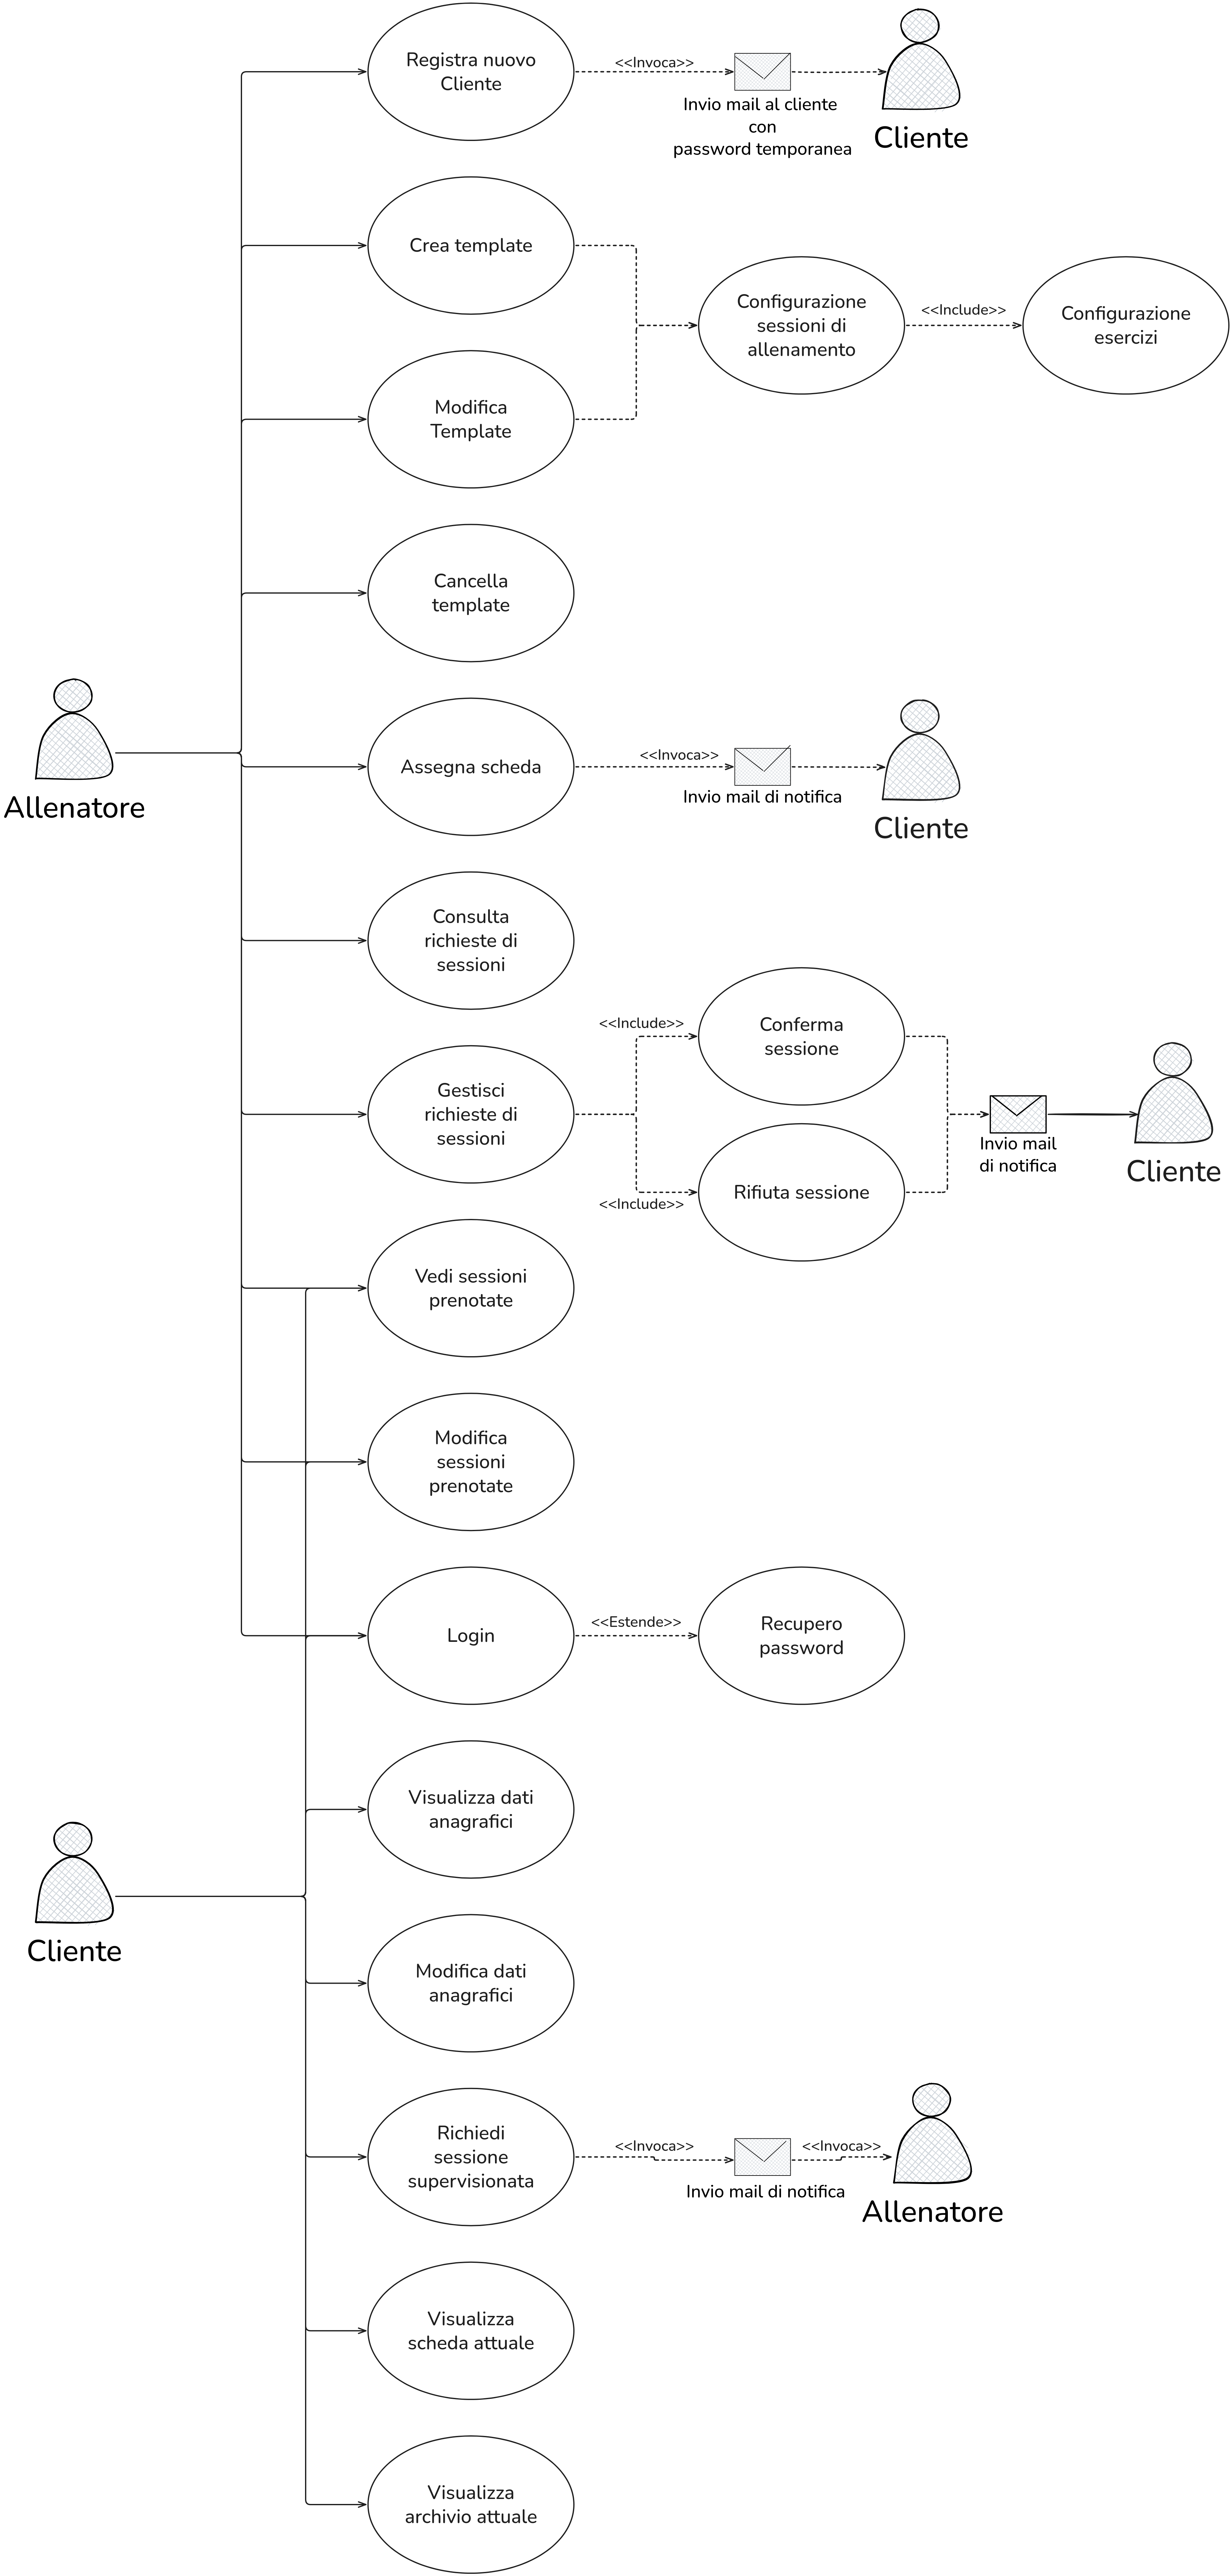
\includegraphics[width=0.5\textwidth]{diagrams/useCaseDiagram.png}
  \caption{Diagramma dei casi d'uso}
  \label{fig:diagrammacasiduso}
\end{figure}

Nel diagramma dei casi d'uso sono rappresentate le interazioni tra
gli attori ed il sistema. Sono presenti alcune azioni che i due
attori hanno in comune, in particolare il login e la
visualizzazione/modifica delle sessioni prenotate.

\subsection{Template dei casi d'uso}
Seguono i template dei casi d'uso comuni a entrambi gli attori:
\subsubsection{U-01: Login}
\subfile{../diagrams/useCaseTemplates/comuni/src/login}

\subsection{Template dei casi d'uso del PT}
Seguono i template dei casi d'uso del PT:
\subsubsection{PT-01: Registrazione PT}
\subfile{../diagrams/useCaseTemplates/allenatore/src/registrazionePT}

\subsubsection{PT-02: Registrazione nuovo Atleta}
\subfile{../diagrams/useCaseTemplates/allenatore/src/creazioneCliente}

\subsubsection{PT-03: Creazione nuova Scheda}
\subfile{../diagrams/useCaseTemplates/allenatore/src/creazioneTemplateScheda}

\subsubsection{PT-04: Configurazione Sessioni di Allenamento in una Scheda}
\subfile{../diagrams/useCaseTemplates/allenatore/src/modificaAllenamentiScheda}

\subsubsection{PT-05: Assegnazione Scheda ad un Atleta}
\subfile{../diagrams/useCaseTemplates/allenatore/src/assegnazioneScheda}

\subsubsection{PT-06: Gestione Richiesta di Sessione di Allenamento}
\subfile{../diagrams/useCaseTemplates/allenatore/src/gestisciRichiesta}

\subsubsection{PT-07: Visualizzazione Sessioni Prenotate}
\subfile{../diagrams/useCaseTemplates/allenatore/src/visualizzazioneSessioniPrenotate}

\subsubsection{PT-08: Visualizzazione Atleti}
\subfile{../diagrams/useCaseTemplates/allenatore/src/visualizzazioneAtleti}

\subsection{Template dei casi d'uso dell'Atleta}
\subsubsection{A-01: Completamento Profilo}
\subfile{../diagrams/useCaseTemplates/cliente/src/registrazioneCliente}

\subsubsection{A-03: Richiesta Sessione di Allenamento}
\subfile{../diagrams/useCaseTemplates/cliente/src/richiestaSessione}

\subsubsection{A-04: Visualizzazione Schede Assegnate}
\subfile{../diagrams/useCaseTemplates/cliente/src/visualizzazioneSchede}

\subsubsection{A-05: Modifica Dati Anagrafici}
\subfile{../diagrams/useCaseTemplates/cliente/src/modificaDatiAnagrafici}

\subsubsection{A-06: Visualizzazione Sessioni Prenotate}
\subfile{../diagrams/useCaseTemplates/cliente/src/visualizzazioneSessioniPrenotate}
